\documentclass[hyperref,german,beleg,noproblem,notoc,plainarticle]{cgvpub}

\usepackage{empheq}

\makeatletter
\def\BState{\State\hskip-\ALG@thistlm}
\makeatother
\DeclareMathOperator*{\argmax}{arg\,max}  % in your preamble
\DeclareMathOperator*{\argmin}{arg\,min}  % in your preamble 

\usepackage{amsmath} % Math packages

%weitere Optionen zum Erg�nzen (in eckigen Klammern):
%
% female	weibliche Titelbezeichnung bei Diplom
% bibnum	numerische Literaturschl�ssel
% final 	f�r Abgabe	
% lof			Abbildungsverzeichis
% lot			Tabellenverzeichnis
% noproblem	keine Aufgabenstellung
% notoc			kein Inhaltsverzeichnis
% twoside		zweiseitig
\author{\textbf{Gruppe 11}\\ Cao,Bozhi\hspace{1em}Gao,Yue\hspace{1em}Jia,Xuehua\hspace{1em}Zhu,Jinyao }
\title{PRAKTIKUMSAUFGABE III}
%\bibfiles{literatur}
%\problem{Text der Aufgabenstellung...}
%\copyrighterklaerung{Hier soll jeder Autor die von ihm eingeholten
%Zustimmungen der Copyright-Besitzer angeben bzw. die in Web Press
%Rooms angegebenen generellen Konditionen seiner Text- und
%Bild"ubernahmen zitieren.}
%\acknowledgments{Die Danksagung..}

\renewcommand\thesection{\arabic{section}.}
\renewcommand\thesubsection{\thesection\arabic{subsection}}
\renewcommand\thefigure{\arabic{figure}}  
\renewcommand\thetable{\arabic{table}}  
\renewcommand{\vec}[1]{\mathbf{#1}}
\setcounter{chapter}{1}
\newcommand*\widefbox[1]{\fbox{\hspace{1em}#1\hspace{1em}}}

\begin{document}

\section{Aufgabe}
\subsection{DAE-System}
Konstitutive Gleichung:
\begin{align*}
\dot{u}_1 &=\frac{1}{C_1} \cdot i_1\\
\dot{u}_2&=\frac{1}{C_2} \cdot i_2
\end{align*} 
Zwangsbedingungen:
\begin{align*}
i_s -i_1 - i_2&=0 \\
u_s - u_R - u_1 &= 0 \\
u_1 - u_2 &= 0 \\
u_R - R \cdot i_s &= 0
\end{align*} 
Definition:
\begin{align*}
x_1 = u_1,\hspace{1em}x_2 = u_2,\hspace{1em}z_1 = i_1,\hspace{1em}z_2 = i_2,\hspace{1em}z_3 = u_R,\hspace{1em}z_4= i_s,\hspace{1em}u = u_s
\end{align*}
$\Rightarrow$semi-explizites DAE-System: 

\begin{empheq}[left={\vec{\dot{x}}=\vec{f}(\vec{z})\Leftrightarrow\empheqlbrace}]{align}
 \dot{x}_1 &= \frac{1}{C_1} \cdot z_1 \label{eq:f1}\\
\dot{x}_2 &= \frac{1}{C_2} \cdot z_2  \label{eq:f2}
\end{empheq}

\begin{empheq}[left={\vec{0}=\vec{g}(\vec{x},\vec{z})\Leftrightarrow\empheqlbrace}]{align}
x_1 - x_2 &= 0 \label{eq:g3}\\ 
u - z_3 -x_1 &=0 \label{eq:g2}\\ 
z_3 - R\cdot z_4 &= 0 \label{eq:g4}\\
z_4 - z_1 - z_2 &= 0 \label{eq:g1}
\end{empheq}
\subsection{Bestimmung des differenziellen Index}
Nach Gl.(\ref{eq:g1}) Gl.(\ref{eq:g2}) und Gl.(\ref{eq:g4}) k"onnen die Variablen $z_3,z_4$ eliminiert werden, die umgeformten Zwangsbedingungen sind:
\begin{empheq}[]{align}
x_1 - x_2 &= 0 \label{eq:ge1}\\ 
u - R \cdot (z_1+z_2) -x_1 &= 0 \label{eq:ge2}
\end{empheq}
offensichtlich aus Gl.(\ref{eq:ge1}) Gl.(\ref{eq:ge2}) kann keine explizite DGL erzeugt werden. $\Rightarrow \mathbf{Index} > 0 $.

\framebox{\textbf{1.Differenziation }}\\
Durch Zeitableitung von Gl.(\ref{eq:ge1}) Gl.(\ref{eq:ge2}) erh"alt man:
\begin{empheq}[]{align}
\dot{x}_1 - \dot{x}_2 &= 0 \label{eq:ged1}\\ 
\dot{u} - R \cdot (\dot{z}_1+\dot{z}_2) - \dot{x}_1 &= 0 \label{eq:ged2}
\end{empheq}
mit Gl.(\ref{eq:f1}) Gl.(\ref{eq:f2}):
\begin{empheq}[]{align}
\frac{1}{C_1} \cdot z_1 - \frac{1}{C_2} \cdot z_2 &= 0 \label{eq:ged3}\\ 
\dot{u} - R \cdot (\dot{z}_1+\dot{z}_2) - \frac{1}{C_1} \cdot z_1 &= 0 \label{eq:ged4}
\end{empheq}
Gl.(\ref{eq:ged3}) in Gl.(\ref{eq:ged4}) einsetzen:
\begin{empheq}[]{align}
\dot{u} - R \cdot (\dot{z}_1+\dot{z}_2) - \frac{1}{C_2} \cdot z_2 &= 0 \label{eq:ged5}
\end{empheq}
bisher ist die Zusammenhang zwischen $\dot{z}_1$ und $\dot{z}_2$ noch unbekannt, deshalb entsteht keine explizite DGL. $ \Rightarrow \mathbf{Index} > 1$.

\framebox{\textbf{2.Differenziation }}\\
Um die Beziehung zwischen $\dot{z}_1$ und $\dot{z}_2$  zu finden, kann man die Gl.(\ref{eq:ged3}) differenzieren:
\begin{empheq}[]{align}
\frac{1}{C_1} \cdot \dot{z}_1 - \frac{1}{C_2} \cdot \dot{z}_2 &= 0 \label{eq:ged6} 
\end{empheq}
setzt man die Gl.(\ref{eq:ged6}) in Gl.(\ref{eq:ged5}) ein:
$$
\dot{u} - R \cdot (\frac{C_1}{C_2}+1)\dot{z}_2 - \frac{1}{C_2} \cdot z_2 = 0 
$$
\begin{empheq}[left={\Rightarrow }]{align}
\dot{z}_2 = -\frac{1}{R\cdot(C_1+C_2)}\cdot z_2 + \frac{C_2}{R\cdot(C_1+C_2)}\cdot \dot{u} \label{eq:ged7} 
\end{empheq}
mit Gl.(\ref{eq:f1}) Gl.(\ref{eq:f2}) Gl.{\ref{eq:ged1}} und Gl.(\ref{eq:ged7}) entsteht ein explizites DGL-System:
\begin{empheq}[left={\vec{\tilde{f}}(z_2,\dot{u})\Leftrightarrow\empheqlbrace}]{align*}
\dot{x}_1 &= \frac{1}{C_2}\cdot z_2 \\
\dot{x}_2 &= \frac{1}{C_2}\cdot z_2 \\
\dot{z}_2 &= -\frac{1}{R\cdot(C_1+C_2)}\cdot z_2 + \frac{C_2}{R\cdot(C_1+C_2)}\cdot \dot{u}
\end{empheq}
jetzt ist der Index des originalen DAE-Systems auf Null reduziert.$\Rightarrow$\framebox{$\mathbf{Index} = 2$}.

Mit den Zwangsbedingungen Gl.(\ref{eq:g1}) Gl.(\ref{eq:g4}) und Gl.(\ref{eq:ged3}) k"onnen die "ubrigen Variablen regeneriert werden:
\begin{empheq}[left={\empheqlbrace }]{align}
z_1 &= \frac{C_1}{C_2}\cdot z_2 \label{eq:ged8} \\
z_4 &= z_1 + z_2 \label{eq:ged9}\\
z_3 &= R\cdot z_4 \label{eq:ged10}
\end{empheq}

\section{Aufgabe}
\subsection{Trapezmethode mit Newton-Rapson-Verfahren}
\textbf{Problemstellung}:\\
Nullstelle von $\boldsymbol{\varphi}_{k+1}(\vec{p}_{k+1})$ iterativ zu finden, wobei:
$$
\boldsymbol{\varphi}_{k+1}(\vec{p}_{k+1}):=
\left( 
\begin{array}{c}
{\varphi}_{1,k+1} \\
{\varphi}_{2,k+1}
\end{array}
\right) 
=\left( 
\begin{array}{c}
\vec{\hat{x}}_{k+1} - \vec{\hat{x}}_{k} - \frac{h}{2}\left[\vec{f}(\vec{\hat{z}}_k) + \vec{f}(\vec{\hat{z}}_{k+1}) \right] \\
\vec{g}(\vec{\hat{x}}_{k+1},\vec{\hat{z}}_{k+1})
\end{array}
\right) 
$$
$$
\vec{p}_{k+1} = \left( \vec{\hat{x}}_{k+1},\vec{\hat{z}}_{k+1}\right)^\top
$$
\textbf{L"osung}:\\
Iterationsvorschrift nach Newton-Rapson-Verfahren:
\begin{align}
\vec{p}_{k+1,i+1}=\vec{p}_{k+1,i}-\vec{J}(\vec{p}_{k+1,i})^{-1}\cdot \boldsymbol{\varphi}_{k+1}(\vec{p}_{k+1,i}) \label{eq:vorschrift}
\end{align}
Iteration "uber $i$ bis:
$$
\|\vec{p}_{k+1,i+1}-\vec{p}_{k+1,i}\|_{\infty}<\varepsilon
$$
wobei $\vec{J}$ ist die Jacobi-Matrix von $\boldsymbol{\varphi}_{k+1}$ an der Stelle $\vec{p}_{k+1,i}$:
\begin{align}
\vec{J}(\vec{p}_{k+1,i})=\left. \frac{\partial \boldsymbol{\varphi}_{k+1}}{\partial \vec{p}_{k+1}}\right|_{\vec{p}_{k+1}=\vec{p}_{k+1,i}} \label{eq:jacobi}
\end{align}
nach Gl.(\ref{eq:f1})$\sim$Gl.(\ref{eq:g4}) und Gl.(\ref{eq:jacobi}), erh"alt man:
\begin{align}
\vec{J} = 
\left( 
\begin{array}{cccccc}
 1 &  0& -\frac{h}{2C_1}&    0&   0&  0 \\
 0 &  1&    0&   -\frac{h}{2C_2}& 0&  0  \\
 1 & -1&    0&      0&   0&  0 \\                      
 1 &  0&    0&      0&   1&  0 \\
 0 &  0&    0&      0&   1& -R \\
 0 &  0&   -1&     -1&   0&  1 
\end{array}
\right) \label{eq:jacobi_matrix}
\end{align}
nach Gl.(\ref{eq:vorschrift}) muss die Jacobi-Matrix invertierbar(regul"ar) sein, deshalb muss:
\begin{align}
\mathrm{det}(\vec{J}(\vec{p}_{k+1,i}))=\frac{h\cdot\left[h+2R\cdot (C_1+C_2)\right] }{4C_1C_2}\neq0 \label{eq:inver_beding}
\end{align}
offensichtlich f"ur jede $h\neq0$ die Bedingung(\ref{eq:inver_beding}) gilt.

\subsection{Bestimmung der Anfangswerten}
Weil es sich um ein Index-2 DAE-System handelt, kann $\vec{x}_0$ und $\vec{z}_0$ nicht frei gew"ahlt werden.\\
Aus der vorgegebenen Bedingung:
$$
\vec{x_0} =
\left( 
\begin{array}{c}
x_{10}\\
x_{20}
\end{array}
\right) 
=
 \vec{0}
$$
mit den Zwangsbedingungen Gl.(\ref{eq:g2}) und Gl.(\ref{eq:ged8})$\sim$(\ref{eq:ged10}), erh"alt man die Anfangswerten von $\vec{z}$:
$$
\vec{z_0} =
\left( 
\begin{array}{c}
z_{10}\\
z_{20}\\
z_{30}\\
z_{40}
\end{array}
\right) 
=
\left( 
\begin{array}{c}
\frac{C_1}{C_1+C_2}\cdot\frac{u_0}{R}\\
\frac{C_2}{C_1+C_2}\cdot\frac{u_0}{R}\\
u_{0}\\
\frac{u_0}{R}
\end{array}
\right) 
$$
\subsection{Analytische L"osung von $u_2(t)$}
Aus dem gegebenen RC-Netzwerk, erh"alt man:
\begin{align*}
(C_1+C_2)\cdot\dot{u}_2(t) &= i_s(t) \\
R\cdot i_s(t) + u_2(t) &= u_s(t)
\end{align*}
\begin{align*}
\Rightarrow \dot{u}_2(t) + \underbrace{\frac{1}{R(C_1+C_2)}}_\tau\cdot u_2(t) = \underbrace{\frac{1}{R(C_1+C_2)}}_\tau \cdot u_s(t)
\end{align*}
L"osung der DGL mit der Anfangsbedingung $u_2(0) = 0$ und $u_s(0) = 10$:
\begin{align*}
u_2(t) = 10\cdot\left( 1 - e^{-\frac{t}{\tau}}\right) 
\end{align*}

\subsection{Kriterium f"ur die numerische Genauigkeit}
Die Singularit"at der Jacobi-Matrix spielt eine wichtige Rolle beim Newton-Raphson-Verfahren f"ur die numerische Genauigkeit der L"osung. Normalerweise, f"ordert man eine hohe numerische Genauigkeit, soll eine m"oglichst kleine Schrittweite verwenden. Aus der Jacobi-Matrix(\ref{eq:jacobi_matrix}), wenn $h\ll1$, sind jedoch die dritte und die vierte Spalte der Jacobi-Matrix fast linear abh"angig, also f"uhrt zu einer singul"aren Jacobi-Matrix. In gewissem Ma"se kann die Determinante der Jacobi-Matrix als ein Kriterium der Singu-larit"at dienen. Im Experiment haben wir gefunden dass, dies ist nicht genug, da eine Matrix kann skaliert beliebig werden, dadurch "andert sich auch die Determinante, aber die Singularit"at hat sich nicht ver"andert. 
Ein besseres Kriterium f"ur die numerische Genauigkeit bzw. die Singularit"at der Jacobi-Matrix ist die \textbf{Konditionszahl} der Jacobi-Matrix. Die Gr"o"se der Konditionszahl beschriebt die Zusammenhang der relativen Fehler an der Ein-und Ausgangsgr"o"se. Eine sehr gro"se Konditionszahl($\mathrm{cond}(\vec{J})\gg1$) impliziert eine hohe Empfindlichkeit der L"osung gegen"uber die Eingangsfehler(z.B. Rundungsfehler bei der 32-Bit-Gleitkommazahl), und f"uhrt zu einer \textbf{schlecht konditionierten} Jacobi-Matrix. Der Solver besitzt deshalb eine schlechte numerische Genauigkeit. Dagegen eine Konditionszahl nahe 1 f"uhrt zu einer \textbf{gut konditionierten} Jacobi-Matrix. In diesem Experiment gibt es ein Dilemma zwischen der Schrittweite und der Konditionszahl der Jacobi-Matrix, welcher die numerische Genauigkeit der Simulation beschrankt.

\subsection{Simulationsergebnisse}
\textbf{Bedingungen}:\\
Fehlerschranke des Newton-Raphson-Verfahrens: 
$$\varepsilon = 1\times10^{-5}$$
Schrittweite der Trapezmethode: 
$$h=1\times10^{-2}\mathrm{s}$$
Simulieren mit Gleitkommazahl einfacher Genauigkeit(32-Bit).

\textbf{Ergebnisse}:
\begin{figure}[!htb]
	\centering
	$
	\begin{array}{cc}
	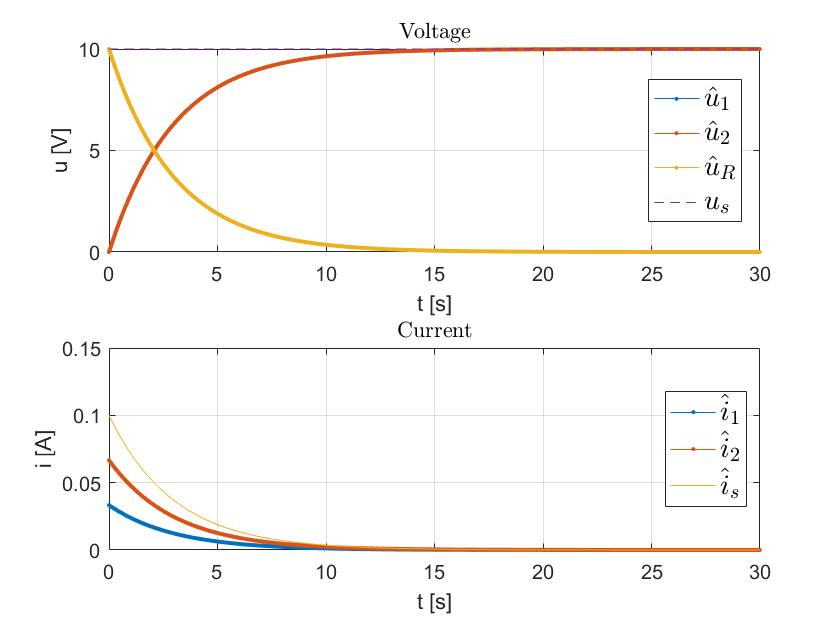
\includegraphics[width=0.43\linewidth]{picture/a2_1} &
	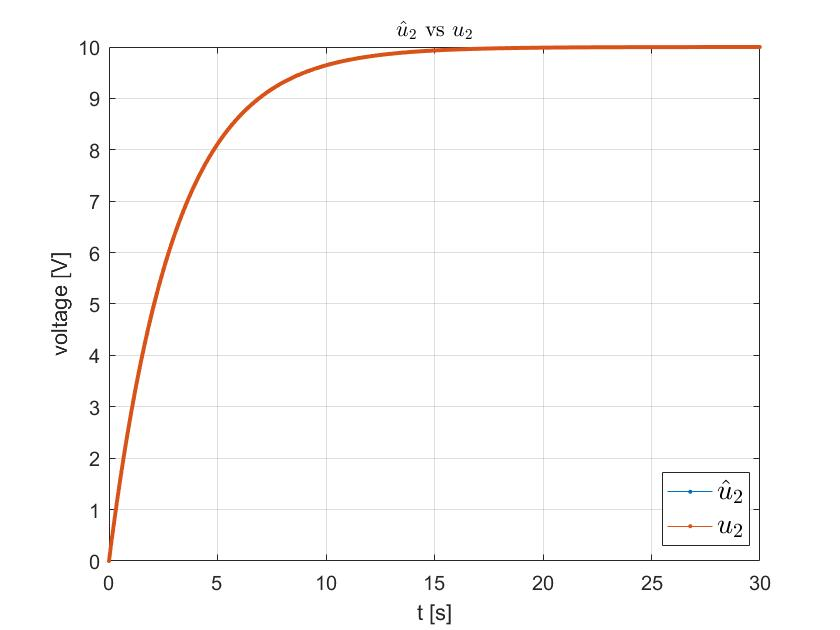
\includegraphics[width=0.43\linewidth]{picture/a2_2}\\
	\text{(a)} &  \text{(b)}\\
	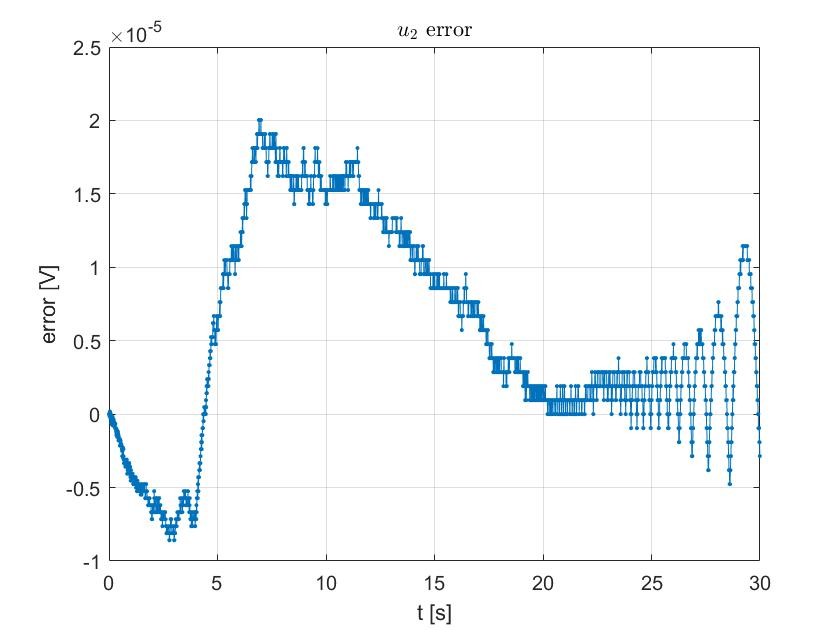
\includegraphics[width=0.43\linewidth]{picture/a2_3} & 
	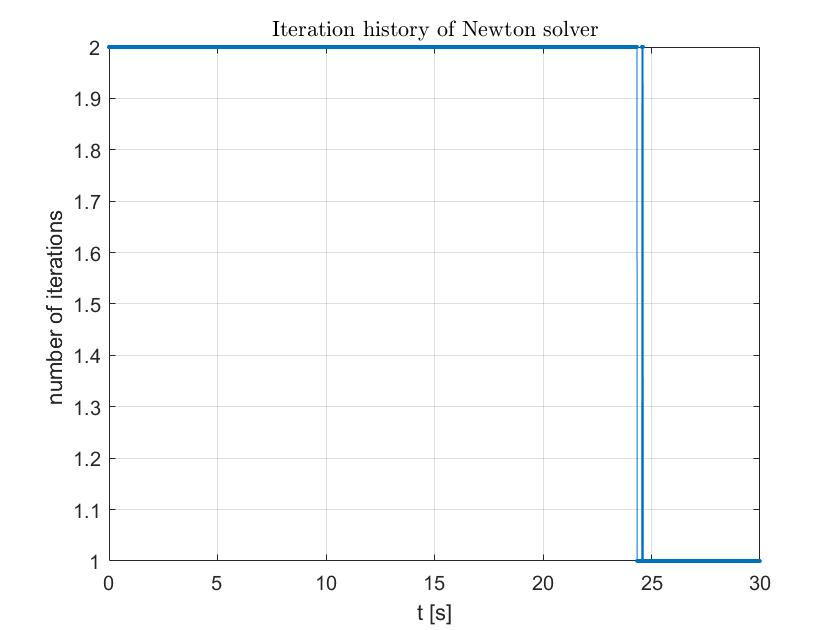
\includegraphics[width=0.43\linewidth]{picture/a2_4} \\
	\text{(c)} & \text{(d)} \\
	\end{array}
	$
	\caption{(a) Verlauf aller Spannungen und Str"ome; (b) Simuliert-/Sollverlauf von $u_2(t)$; (c) Differenz zum Sollverlauf von $u_2(t)$; (d) Verlauf der Iterationsschritte beim Newton-Raphson-Verfahren;}
	\label{fig1}
\end{figure}
\newpage
\textbf{Untersuchung der numerischen Genauigkeit}:
\begin{figure}[htb]
	\centering
	$
	\begin{array}{cc}
	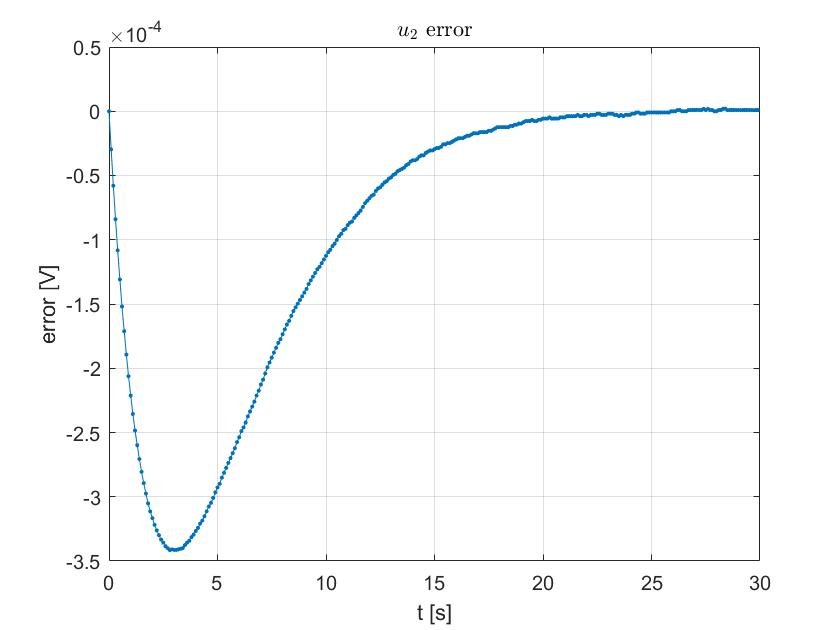
\includegraphics[width=0.43\linewidth]{picture/a2_5} &
	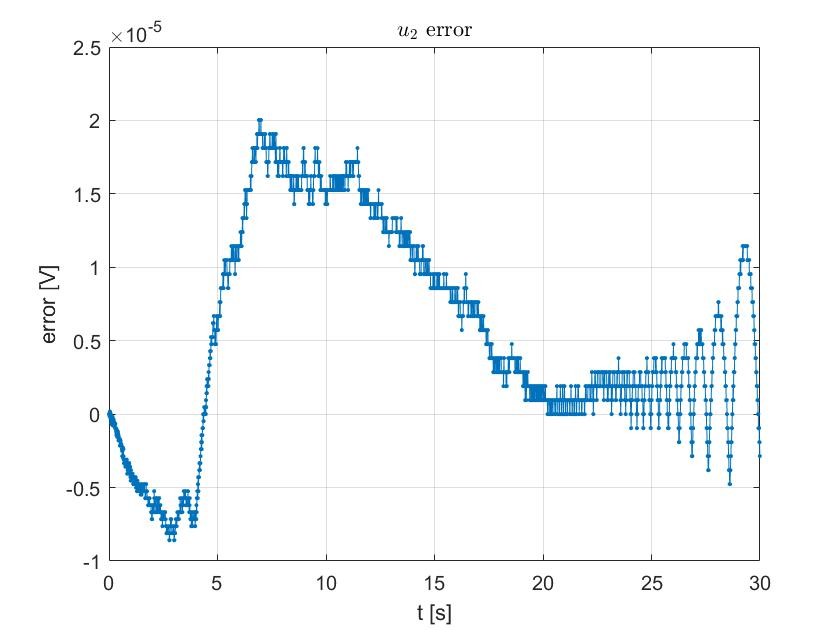
\includegraphics[width=0.43\linewidth]{picture/a2_3}\\
	\text{(a)} &  \text{(b)}\\
	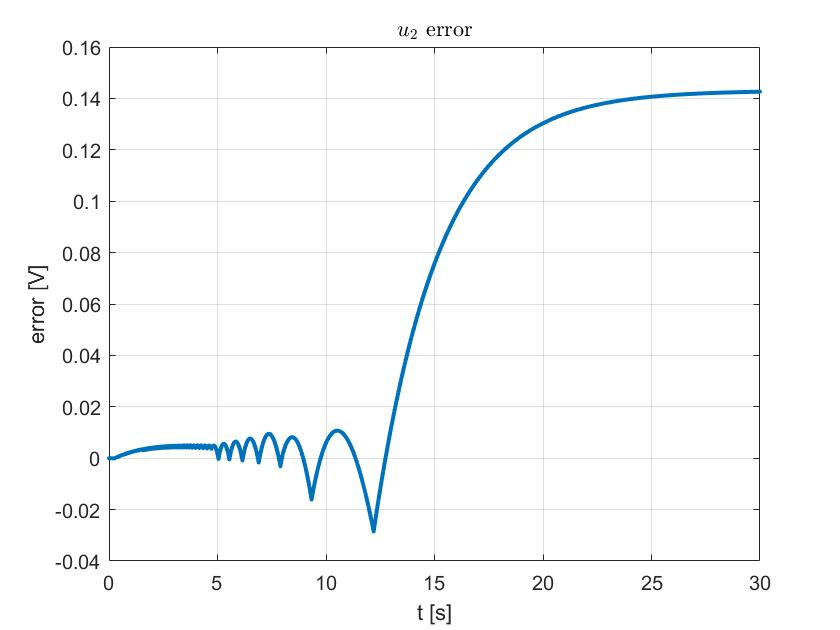
\includegraphics[width=0.43\linewidth]{picture/a2_6} & 
	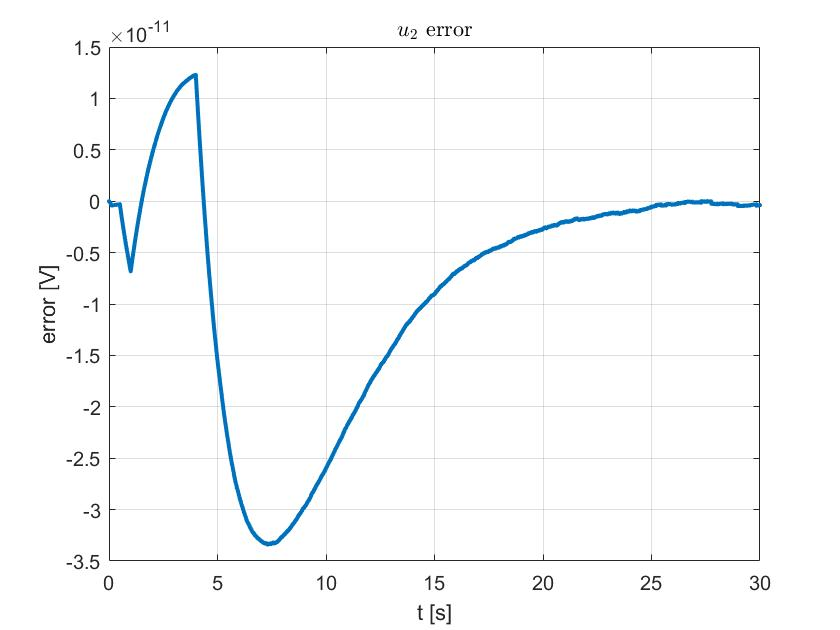
\includegraphics[width=0.43\linewidth]{picture/a2_7} \\
	\text{(c)} & \text{(d)} \\
	\end{array}
	$
	\caption{(a) $h = 1\times10^{-1}\mathrm{s}$, einfache Genauigkeit; (b) $h = 1\times10^{-2}\mathrm{s}$, einfache Genauigkeit; (c) $h = 1\times10^{-5}\mathrm{s}$, einfache Genauigkeit; (d) $h = 1\times10^{-5}\mathrm{s}$, doppelte Genauigkeit;}
	\label{fig2}
\end{figure}
\begin{table}[!h]
\centering
\begin{tabular}{c||c|c|c|c}
    \hline 
  $h$ [s] 	& Datentype &$\mathrm{det}(\vec{J})$ & $\mathrm{cond}(\vec{J})$ & max. ||error|| [V] \\ 
	\hline 
  $1\times10^{-1}$ & single & 762.5 & 327.9 & $3.4\times10^{-4}$\\ 
	\hline 
  $1\times10^{-2}$ & single & 75.13 & 339.1 & $2.0\times10^{-5}$\\ 
	\hline 
 $1\times10^{-5}$ & single	& 0.075 & $3.3\times10^{5}$ & \framebox{0.142} !!!\\ 
	\hline 
 $1\times10^{-5}$ & double	& 0.075 & $3.3\times10^{5}$ & $3.3\times10^{-11}$\\ 
\hline 
\end{tabular} 
\caption{Numerische Genauigkeit, $\mathrm{cond}(\vec{J})$ = (2-Norm)Konditionszahl der Jacobi-Matrix}
\end{table}\\
Aus den Simulationsergebnisse kann man sehen, dass bei sehr kleinen Schrittweite($h=1\times10^{-5}\mathrm{s}$) verschlechtert sich der numerische Genauigkeit dramatisch. Die Rundungsfehler der Gleitpunktzahl werden sich von der schlecht konditionierten Jacobi-Matrix erheblich vergr"o"sert.\\
Nach mehreren Versuche haben wir gefunden, dass bei $h\approx1.3\times10^{-2}\mathrm{s}$ besitzt die Simulation(mit einfacher Gleitkommazahl) eine h"ochst numerische Genauigkeit von max. ||error||
$\approx1.05\times10^{-5}$ V.
\end{document}